\subsection{Resumo}

\begin{table}[h!]
\centering
\begin{tabular}{ |c|c|c|c|c|  }
\hline
\rowcolor{lightgray}
Algoritmo & Max & Min & Média & Desvio Padrão \\
\hline
Hill-Climbing & 20360.232 & 18608.415 & 19652.804 & 621.752 \\
\hline
Hill-Climbing com restart & 20708.751 & 19393.573 & 19898.23 & 394.147 \\
\hline
Simulated Annealing & 20280.727 & 18859.27 & 19694.674 & 505.547 \\
\hline
Genetic Algorithm & 18577.383 & 15538.484 & 16879.374 & 1006.5 \\
\hline

\end{tabular}
\caption{Tabela com dados consolidados dos algoritmos}
\end{table}

\begin{figure}[H]
\centering
  \begin{minipage}[b]{0.48\textwidth}
    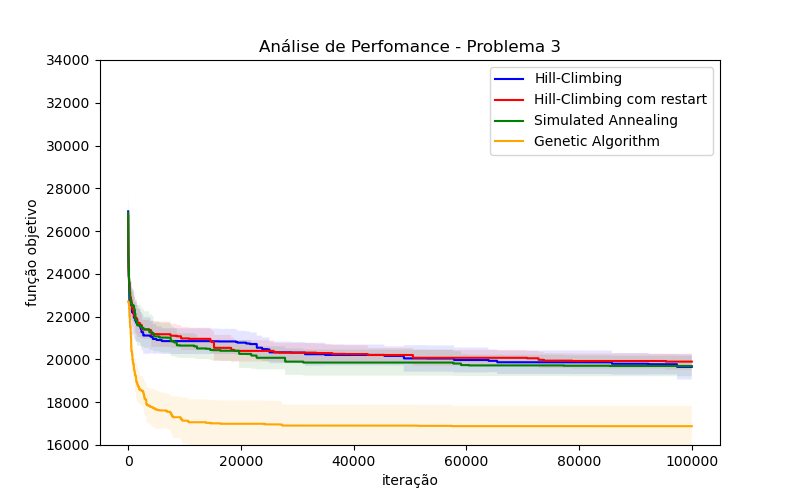
\includegraphics[width=88mm]{imagens/otima/problema-3-performance-algoritmos-best.png}
    \caption{Dados da execução da função objetivo durante as 10 iterações por melhor valor.
    \label{fig:problema-3-performance-algoritmos-best}}
  \end{minipage}
  \hfill
  \begin{minipage}[b]{0.48\textwidth}
    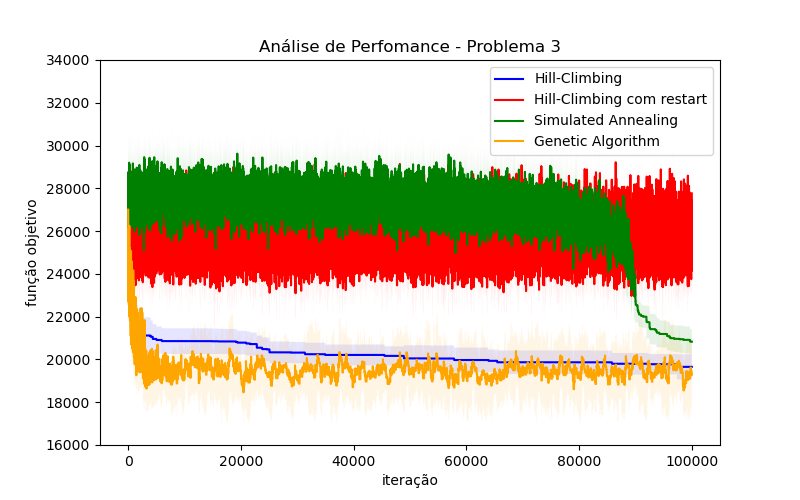
\includegraphics[width=88mm]{imagens/otima/problema-3-performance-algoritmos-value.png}
    \caption{Dados da execução da função objetivo durante as 10 iterações por valor atual.
    \label{fig:problema-3-performance-algoritmos-value}}
  \end{minipage}
\end{figure}